As described in Section~\ref{sec:data} of the main text, PGE offers 23 distinct agricultural tariffs, which fall into 5 categories, depending on a farmer's meter type (conventional vs. smart) and pumping capital (small, large, or previously powered by an internal combustion engine). Here, we present additional details on these rates. Table~\ref{tab:pge_ag_tariffs} describes each rate in detail, including a description of the eligibility category, the broad pricing schedule on each rate, and the share of customers on each rate within our sample. Figure~\ref{fig:marg_price_all_rates} shows a time series of each rate over our sample. This is analogous to Figure~\ref{fig:marg_price_5_default_rates} in the main text, but shows all rates in addition to the ``default'' within-category rate. All rates that are the same color in Figure~\ref{fig:marg_price_all_rates} belong to the same category; the default rate for each category is bolded. The left panel shows the raw rate time series. The right panel shows residualized rates, after partialling out tariff $\times$ month-of-year fixed effects and month-of-sample fixed effects. 
\\
\\

\begin{figure}[h!]\centering
\captionsetup{width=\textwidth}
\caption{Average marginal electricity prices (all rates)}
\label{fig:marg_price_all_rates}
\vspace{-2mm}
{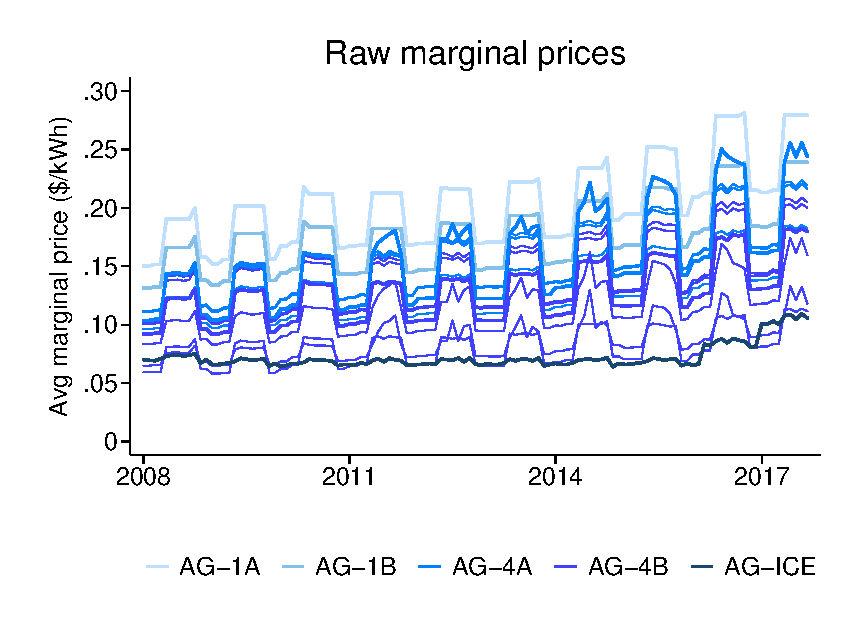
\includegraphics[width=.495\textwidth]{figures/marg_price_all_rates_raw_wtitle.eps}}~
{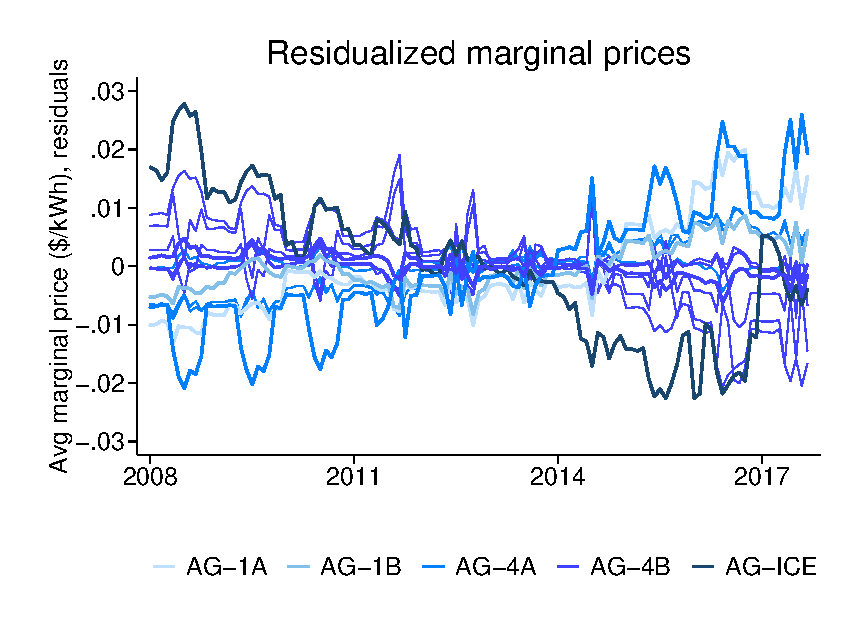
\includegraphics[width=.495\textwidth]{figures/marg_price_all_rates_resid_wtitle.eps}}
\\
\captionsetup{width=\textwidth}
\caption*{\scriptsize \emph{Notes:} This figure plots times series of monthly average marginal electricity prices (\$/kWh) for all of PGE agricultural tariffs. These 23 tariffs are divided into 5 mutually-exclusive categories, based on the type of electricity meter on a farm (smart vs. conventional) and a farm's pumping capital (small, large, or previously internal combustion engine). All rates belonging to the same category are the same color. The five ``default'' rates, which we also show in main text Figure~\ref{fig:marg_price_5_default_rates} are bolded. The left panel plots raw average marginal prices for each month in our estimation sample, taking unweighted averages across all hours. The right panel plots residuals of these same five time series, after partialling out tariff $\times$ month-of-year fixed effects and month-of-sample fixed effects (aligning with the fixed effects we use in estimation). AG-1A and AG-1B are non-time-varying rates (i.e.\ constant marginal price for all hours within a month), whereas AG-4A and AG-4B are time-varying rates (i.e.\ higher marginal prices during peak hours and weekdays). AG-1A and AG-4A are for small pumps ($<35$ hp), whereas AG-1B and AG-4B are for large pumps ($\ge35$ hp). AG-ICE is a time-varying rate for customers with auxiliary internal combustion engines. Marginal prices are systematically higher during summer months (May--October). Our identifying variation comes (a) strict restrictions that segment customers into categories; (b) the fact that the residualized default prices do not move in parallel; and (c) PGE's smart meter rollout, which exogenously shifted many customers from the AG-1A/1B default tariffs to the AG-4A/4B default tariffs with lower marginal prices.}
\end{figure}
\begin{table}[b!]\centering
\footnotesize
\caption{PGE agricultural tariffs}
\label{tab:pge_ag_tariffs}
\vspace{-2mm}
\begin{adjustbox}{center}
\begin{tabular}{|c|c|c|c|}
\hline
\textbf{Category} & \textbf{Tariff} & \textbf{ Description} & \textbf{ Percent} \\
\hline
$ \begin{matrix}
\text{\bf Small pumps, conventional meters} \\
\text{single motor $<35$ hp, or} \\
\text{multiple motors summing to $<15$ hp}
\end{matrix} $
 & \textbf{1A} &  
\footnotesize $ \begin{matrix}
\text{High price per kWh (not time-varying),} \\
\text{fixed charge per hp connected} \\
\end{matrix} $ &  3.0 \\
\hline
$ \begin{matrix}
\text{\bf Large pumps, conventional meters} \\
\text{single motor $\ge 35$ hp, or} \\
\text{multiple motors summing to $\ge15$ hp,} \\
\text{or single overloaded motor $\ge 15$ hp}
\end{matrix} $ & \textbf{1B} &
\footnotesize $ \begin{matrix}
\text{High price per kWh (not time-varying),} \\
\text{fixed charge per max kW consumed} \\
\end{matrix} $ &  8.1 \\
\hline
\multirow{4}{*}{
$ \begin{matrix} \\ \\ \\ \\
\text{\bf Small pumps, smart meters} \\
\text{single motor $<35$ hp, or} \\
\text{multiple motors summing to $<15$ hp}
\end{matrix} $ 
} & \textbf{4A} (4D) & 
\footnotesize $ \begin{matrix}
\text{High prices per kWh (higher in peak hours),} \\
\text{fixed charges per hp connected, } \\
\text{very high peak prices on 14 summer Event Days} \\
\end{matrix} $ &  7.2 \\
\cline{2-4}
 & 5A (5D) &
\footnotesize $ \begin{matrix}
\text{Lower prices per kWh (peak \& offpeak),} \\
\text{no Event Day price increases, } \\
\text{higher fixed charges per hp} \\
\end{matrix} $ &  2.7 \\
\cline{2-4}
&  RA (RD) & 
\footnotesize $ \begin{matrix}
\text{Lower peak prices per kWh,} \\
\text{higher off-peak prices per kWh,} \\
\text{no Event Day price increases, } \\
\text{choice between MTW or WTF peak days} \\
\end{matrix} $ &  1.2 \\
\cline{2-4}
& VA (VD) & 
\footnotesize $ \begin{matrix}
\text{Lower peak prices per kWh,} \\
\text{higher off-peak prices per kWh,} \\
\text{no Event Day price increases, } \\
\text{choice of 3 shorter 4-hour peak periods} \\
\end{matrix} $ &  0.9 \\
\hline
\multirow{6}{*}{
$ \begin{matrix} \\ \\ \\ \\ \\ \\
\text{\bf Large pumps, smart meters} \\
\text{single motor $\ge 35$ hp, or} \\
\text{multiple motors summing to $\ge15$ hp,} \\
\text{or single overloaded motor $\ge 15$ hp}
\end{matrix} $
} & \textbf{4B}  (4E) & 
\footnotesize $ \begin{matrix}
\text{High prices per kWh (higher in peak hours),} \\
\text{fixed charges per max kW consumed} \\
\end{matrix} $ &  20.1 \\
\cline{2-4}
&  5B (5E) & 
\footnotesize $ \begin{matrix}
\text{Much lower prices per kWh (peak \& offpeak),} \\
\text{higher fixed charge per max kW} \\
\end{matrix} $ &  37.8 \\
\cline{2-4}
 & 4C (4F) &
\footnotesize $ \begin{matrix}
\text{Slightly lower prices per kWh (peak \& offpeak),} \\
\text{higher fixed charges per kW shifted to peak,} \\
\text{very high peak prices on 14 summer Event Days} \\
\end{matrix} $ &  2.4 \\
\cline{2-4}
& 5C (5F) &
\footnotesize $ \begin{matrix}
\text{Much lower prices per kWh (peak \& offpeak),} \\
\text{higher fixed charges per kW shifted to peak,} \\
\text{very high peak prices on 14 summer Event Days} \\
\end{matrix} $ &  7.8 \\
\cline{2-4}
& RB (RE) & 
\footnotesize $ \begin{matrix}
\text{Higher prices per kWh (peak \& off-peak),} \\
\text{choice between MTW or WTF peak days,} \\
\text{lower fixed charges per max kW (in summer)} \\
\end{matrix} $ &  1.5 \\
\cline{2-4}
& VB (VE) & 
\footnotesize $ \begin{matrix}
\text{Higher prices per kWh (peak \& off-peak),} \\
\text{choice of 3 shorter 4-hour peak periods,} \\
\text{lower fixed charges per max kW (in summer)} \\
\end{matrix} $ &  0.6 \\
\hline
$ \begin{matrix}
\text{\bf Customers transitioning off} \\
\text{\bf internal combustion engines}
\end{matrix} $
 & \textbf{ICE} & 
\footnotesize $ \begin{matrix}
\text{Very low price per kWh (high in peak hours),} \\
\text{fixed charge per max kW consumed} \\
\end{matrix} $ & 6.8 \\
\hline
\end{tabular}
\end{adjustbox}
 \captionsetup{width=1.1\textwidth}
\caption*{\scriptsize \emph{Notes:}
This table provides a rough summary of PGE's 23 electricity tariffs for agricultural customers. 
The first column lists the 5 disjoint categories of customers, defined (primarily) by physical pumping capital and electricity meters.
Effective default tarrifs within each group are in bold, and farmers may switch tariffs \emph{within} a category (but not \emph{across} categories).
All tariffs have fixed (\$/kW) and volumetric (\$/kWh) prices that vary by summer vs.\ winter. 
All time-of-use tariffs (i.e. all but 1A and 1B) also vary between peak (12:00pm--6:00pm on summer weekdays), partial peak (8:30am--9:30pm on weekends), and off-peak periods.
DEF tariffs are functionally equivalent to their ABC analogs, and are holdovers for the earliest customers to adopt time-of-use pricing.
Actual tariffs are far more complex, and tariff documents are available at \url{https://www.pge.com/tariffs/index.page}.
The right-most column reports the percent of observations in our main estimation sample on each tariff.
}
\end{table}
\FloatBarrier
